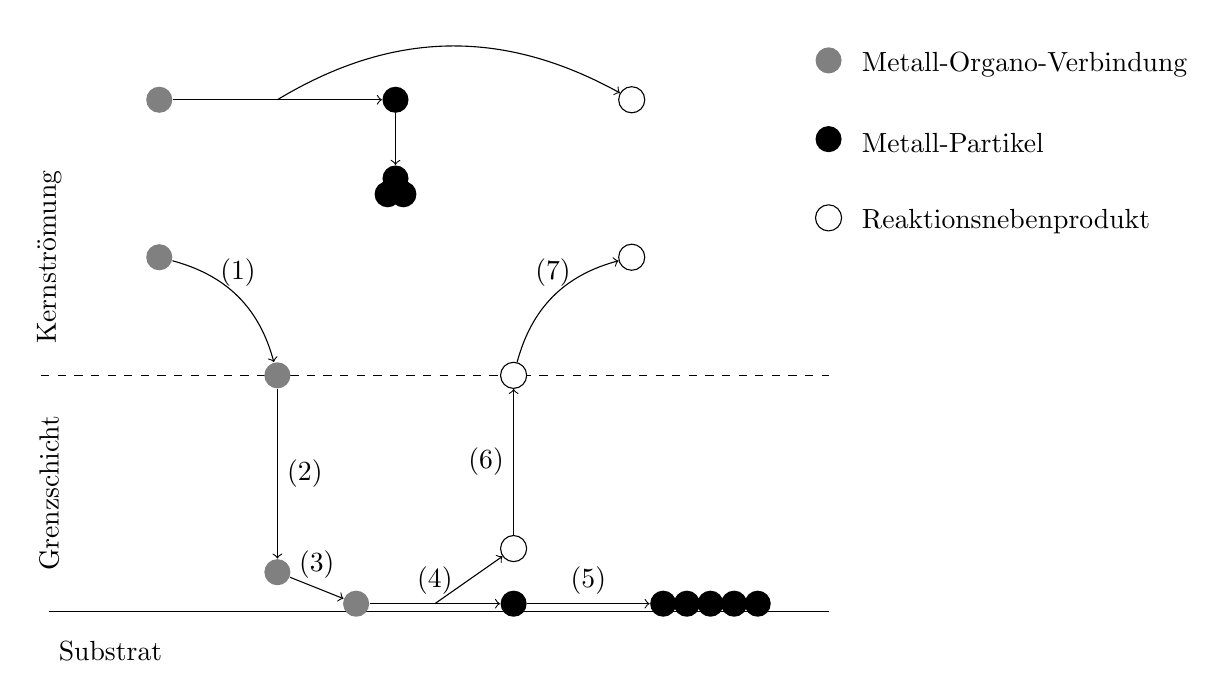
\begin{tikzpicture}
% Schritte 1-7
% Linien und Bereiche
\draw[color = black,dashed](-6,3) -- (4,3);
\node[rotate = 90]at(-5.9,4.5){Kernstr\"omung};
\node[rotate = 90]at(-5.9,1.5){Grenzschicht};
\draw[color = black](-5.9,0) -- (4,0);
\node[anchor=west]at(-5.9,-0.5){Substrat};
% Bezeichnung
\node[black,fill=gray,circle]at(4,7) (){};
\node[anchor=west]at(4.3,6.95)(grau_schrift){Metall-Organo-Verbindung};
\node[black,fill=black,circle]at(4,6) (){};
\node[anchor=west]at(4.3,5.95)(grau_schrift){Metall-Partikel};
\node[black,fill=white,circle,draw]at(4,5) (){};
\node[anchor=west]at(4.3,4.95)(grau_schrift){Reaktionsnebenprodukt};

% Partikel
\node[black,fill=gray,circle]at(-4.5,4.5) (bulk){};
\node[black,fill=gray,circle]at(-3,3) (grenze1){};
\node[black,fill=gray,circle]at(-3,0.5) (ads){};
\node[black,fill=gray,circle]at(-2,0.1)(surface){};
\node[black,fill=black,circle]at(0,0.1)(surface_metall){};
\node[black,circle,draw]at(0,0.8)(surface_organo){};
\node[black,fill=white,circle,draw]at(0,3)(grenze_organo){};
\node[black,fill=white,circle,draw]at(1.5,4.5) (bulk_organo){};
% Metallzentrum
\node[black,fill=black,circle]at(1.9,0.1)(MZ_l){};
\node[black,fill=black,circle]at(2.2,0.1)(MZ_m1){};
\node[black,fill=black,circle]at(2.5,0.1)(MZ_m2){};
\node[black,fill=black,circle]at(2.8,0.1)(MZ_m3){};
\node[black,fill=black,circle]at(3.1,0.1)(MZ_r){};
% Pfeile
\draw[black,->,bend left, bend angle = 10](bulk)to node[above]{$(1)$}(grenze1);
\draw[black,->](grenze1) to node[right]{$(2)$}(ads);
\draw[black,->](ads) to node[above]{$(3)$}(surface);
\draw[black,->](surface) to node[above]{$(4)$}(surface_metall);
\draw[black,->](-1,0.1) to (surface_organo);
\draw[black,->](surface_metall) to node[above]{$(5)$}(MZ_l);
\draw[black,->](surface_organo) to node[left]{$(6)$}(grenze_organo);
\draw[black,->,bend left, bend angle = 10](grenze_organo)to node[above]{$(7)$}(bulk_organo);

% Gasphasenreaktion
\node[black,fill=gray,circle]at(-4.5,6.5) (bulk2){};
\node[black,fill=white,circle,draw]at(1.5,6.5) (bulk_organo2){};
\node[black,fill=black,circle]at(-1.5,6.5) (bulk_metall){};
\node[black,fill=black,circle]at(-1.5,5.5) (bulk_metall2){};
\node[black,fill=black,circle]at(-1.6,5.3) (bulk_metall3){};
\node[black,fill=black,circle]at(-1.4,5.3) (bulk_metall4){};
\draw[black,->](bulk2) to (bulk_metall);
\draw[black,->](bulk_metall) to (bulk_metall2);
\draw[black,->,bend left, bend angle = 45](-3,6.5)to(bulk_organo2);
\end{tikzpicture}